%!TEX root=Principal.tex
\chapter{CONCEITOS FUNDAMENTAIS}
\label{cap:ai}
Este capítulo apresenta os conceitos fundamentais das técnicas utilizadas para desenvolvimento da tese apresentada.

\section{Agrupamento de Dados}
\label{sec:clustering}
Encontrar padrões em informações do mundo real é uma tarefa complexa. O conhecimento sobre o domínio de aplicação ou dos fenômenos naturais é imprescindível na maioria dos casos. Sem esse conhecimento, gerar modelos e padrões matemáticos para compreender os efeitos de tal fenômeno ou aplicação no mundo é complicado~\cite{kantardzic:2011}.

Com o avanço da tecnologia e sua popularização ocorreu um aumento na criação de informações, sendo este sem ordem ou normalização. O mundo coorporativo enxergou nesse fenômeno uma potencial fonte de conhecimento. Porém, encontrar padrões ou modelos que torne possível encontrar conhecimento nessas informações não é uma tarefa trivial. A partir desse problema, pesquisadores começaram a desenvolver técnicas e algoritmos computacionais onde houvesse então a mineração dos dados, como ficou conhecida a técnica~\cite{jain:1999, kantardzic:2011}.

Minerar dados é um processo realizado com dois objetivos. Predição da informação, onde é possível prever o futuro com base em algumas informações coletadas. E descrição da informação, que apresenta um rótulo mais compreensível ao ser humano a partir dos padrões encontrados nos dados coletados~\cite{jain:1999}.

Dentro do processo de mineração de dados existe um passo chamado de agrupamento de dados. O agrupamento de dados é fundamental para, a partir de um volume finito de informação, extrair padrões e forma grupos com base na similaridade encontrada em cada registro. A extração dos padrões tem como base algumas técnicas aplicadas para associação e classificação. O resultado final dos padrões encontrados pode variar dependendo das técnicas aplicadas~\cite{kantardzic:2011, witten:2011}. As técnicas existentes são:

\begin{itemize}
    \item \textbf{Exclusivo}: os elementos pertencem a um grupo apenas;
    \item \textbf{\emph{Overlaping}}: os elementos podem pertencer a mais de um grupo, simultâneamente;
    \item \textbf{Probabilístico}: os elementos possuem um grau probabilidade de pertencer a um grupo;
    \item \textbf{Hierárquico}: realiza a divisão aproximada dos grupos. Refina a divisão encontrada até que alcance um resultado que não se altere muito entre as iterações.
\end{itemize}

O maior desafio da técnica de agrupamento de dados é a maneira de tratar e associar os diversos tipos de informação existentes com por exemplo, números, textos e imagens. Além disso, as informações podem ser extraídas de maneira qualitativa ou quantitativa~\cite{witten:2011}. A seção~\ref{sec:algoritmosclustering} apresentará alguns dos principais algoritmos de agrupamento de dados existentes.

\subsection{Algoritmos de Agrupamento de Dados}
\label{sec:algoritmosclustering}
Para realizar o agrupamento de informações existem diversos algoritmos. Alguns dos algoritmos mais populares e outros com aplicações mais específicas serão apresentados nessa seção.

Dentre os algoritmos existentes o mais popular é o k-means. Ele utiliza da distância eucliana para comparar a similaridade entre os dados, tentando minimizar o erro quadrático. A partir do momento que o erro não tiver mais alterações entre as iterações do algoritmo, ele encerra o processo de agrupamento. Ele precisa que o número de grupos desejados seja informado e realiza uma inicialização de sementes, para cada grupo, de maneira aleatória. Devido a isso, o resultado do agrupamento pode ser diferente entre as execuções do algoritmo. O resultado do k-means é bem consistente, mas mesmo para apenas dois grupos, encontrar a solução ótima com o k-means é um processo considerado NP-\emph{Hard}~\cite{jain:2010, witten:2011}.

\emph{Graph-based Clustering} (GBC) é um algoritmo de agrupamento baseado na teoria de grafos. Ele liga uma aresta entre os dados e o ponto médio entre as arestas é utilizado para determinar a divisão dos grupos de maneira automática. O problema apresentado pelo GBC é na concentração densa dos dados. Quando ocorre esse tipo de cenário, o algoritmo acaba considerando todos os dados pertencentes a um único grupo~\cite{muhlenbach:2009}.

Outro algoritmo existente é o \emph{Quick ROCK} (QROCK) que tem como objetivo o agrupamento de informações categóricas, ou seja, informações textuais. Ele é um algoritmo de agrupamento hierárquico aglomerativo. Assim como o GBC ele determina o resultado com base na conexão dos elementos através de um grafo. Para determinar a quantidade de grupos é necessário informar um valor de corte $\theta$ representando o valor de similiaridade entre os dados. Esse valor é calculado com base na equação~\ref{eq:sim_qrock} e tende a deixar o agrupamento mais natural~\cite{dutta:2005}.

\begin{equation}
    \label{eq:sim_qrock}
    SIM(X, Y) = \frac{X \bigcap Y}{X \bigcup Y}
\end{equation}

Com o foco em agrupamento de informações espaciais, o algoritmo \emph{Density Based Spacial Clustering of Applications with Noise} (DBSCAN) foi apresentado por~\citeonline{ester:1996}. Para realizar o processo de agrupamento, são necessários dois parâmetros. Distância mínima entre dois pontos, que auxilia ao dizer se os pontos fazem parte ou não do mesmo grupo. E o outro parâmetro é a quantidade mínima de pontos para formar um grupo. Esse último parâmetro é importante para determinar se existirá um grupo ou se alguns pontos serão considerados como ruídos e desconsiderados do resultado final. Com base de dados espaciais em duas dimensões o DBSCAN conseguiu segmentar bem as diferentes regiões existentes, porém com dados de dimensões maiores isso já não foi possível.

\emph{Affinity Propagation} é um algoritmo de agrupamento sem necessidade de informar qualquer parâmetro para o processo. Ele considera todos os dados como potenciais centróides de grupos. E como uma rede neural de aprendizado competitivo, vai identificando os dados que possuem mais arestas e determinando os grupos com base nestes. Seu desempenho é considerado bom apenas quando o resultado inicial está próximo do ótimo~\cite{frey:2007}.

Perfis de usuários são compostos de diversos tipos de informação. Isso torna o processo de agrupamento mais complexo, pois é necessário criar uma regra de similaridade que atenda cada tipo de informação e também consiga estipular um valor único por perfil. Com esse problema em mente o algoritmo \emph{Quality Groups of Similarity Clustering} (QG-SIM) foi criado. É necessário informar o valor $q$ que representa a similaridade mínima para manter entre os elementos do grupo. Apesar de ser útil em diversas aplicações, o enfoque dele é em aplicações de perfis de usuários. Um ponto fraco dele é o desempenho computacional que depende da quantidade de dados dentro de cada um dos grupos~\cite{masiero:2013}.

A tabela~\ref{tab:comp_algo_agrupamento} apresenta uma comparação entre os algoritmos de agrupamento de dados e suas principais características.

\begin{table}[h!]
	\caption{Tabela comparativa entre os algoritmos}
	\label{tab:comp_algo_agrupamento}
	\begin{tabular}{ m{2.8cm} | m{5cm} | m{7cm} } \hline
	Categoria & Algoritmo & Parâmetro / Propriedades \\ \hline
	\emph{clustering} hierárquico & Ward & algoritmo aglomerativo \\ \hline
	& MST Divisivo & baseado na teoria de grafos \\ \hline
	& \emph{Clustering Using REpresentatives (CURE)} & cada grupo é representado por um conjunto de representações \\ \hline
	& \emph{RObust Clustering using linKs (ROCK)} & $k*$: número de grupos \\ \hline
	& QROCK (\emph{Quick} ROCK) & $\theta$: \emph{threshold} de similaridade  \\ \hline
	\emph{hard clustering} & $k$\emph{means} & $k*$: número de grupos \\ \hline
    & QG-SIM & $q$: similaridade mínima entre os elementos do grupo \\ \hline
	\emph{clustering} baseado em densidade & DBSCAN & $\epsilon$: distância para considerar se 2 pontos são ou não vizinhos \\ \hline
	& \emph{Affinity Propagation} & $\theta$: \emph{threshold} de similaridade  \\ \hline
	\emph{clustering} sequencial & \emph{Basic Sequential Algorithm Scheme (BSAS)} & $\Theta$: \emph{threshold} de não similaridade e $k*$: número máximo de grupos  \\ \hline
	\end{tabular}
	\smallcaption{Fonte: Adaptada de \citeonline{muhlenbach:2009}.}
\end{table}

Nesta tese, como há um trabalho de agrupamento de perfil de usuário, optou-se por utilizar o algoritmo QG-SIM que foi, de acordo com a literatura, o que apresentou melhores resultados para identificar qual a quantidade de perfis na população de acordo com o critério de grupo, considerando a técnica de Personas~\cite{masiero:2013}.

\section{Raciocínio Probabilístico}
\label{sec:raciocinio-probabilistico}
Para que um agente possa tomar uma decisão, é necessário que ele analise todas as possibilidades de ações que possam ser feitas e o que ocorrerá após a tomada de decisão para que exista uma certeza sobre o caminho que deve ser seguido. O processo para encontrar a certeza sobre uma decisão, computacionalmente, é oneroso e consome muito tempo para alcançar um resultado. A quantidade de variáveis geralmente consideradas na solução destes problemas também é grande, tornando-se inviável a busca pela solução com 100\% de certeza. Sendo assim, um agente precisa trabalhar com a incerteza sobre o domínio para que possa ser tomada uma decisão~\cite{russell:2002}.

Fazer o agente tomar uma decisão considerando a incerteza, é fazer o agente manter o controle baseado em um estado de crença, em outras palavras, um conjunto com todos os possíveis estados em um domínio ao qual ele possa estar. Além disso, o agente deve prever e gerar um plano de contingência para eventuais situações que sejam detectadas durante a execução do algoritmo. Nesses problemas, as informações que o agente possui não conseguem garantir nenhum resultado com certeza absoluta. Porém, tais informações garantem um grau de crença de que o objetivo será alcançado ou a decisão de um caminho relevante a ser tomada~\cite{russell:2002, faceli:2011}.

Todas as declarações feitas com base na crença sobre as informações não se contradizem mutuamente. Cada uma é uma afirmação separada de um diferente estado de conhecimento. Cada vez que é inserida uma informação nova e complementar, é aumentado o estado de crença sobre um determinado assunto, melhorando a tomada de decisão do agente~\cite{faceli:2011}.

Para que a tomada de decisão tenha uma maior utilidade ao agente, ele deve ter preferências dentre os diferentes resultados apresentados. Sendo assim, ter uma decisão com base apenas na probabilidade, não é recomendável. Essa é a base da teoria da utilidade. A teoria da utilidade é utilizada para que o agente represente e raciocine em seu problema, de acordo com suas preferências. É distribuido um grau de utilidade para cada escolha que o agente possa ter, assim o estado que possui o maior grau de utilidade é escolhido. Pode-se dizer então que uma decisão é tomada com base na probabilidade de um estado somado a sua utilidade~\cite{russell:2002}.

Utilizar as teorias de probabilidade e utilidade, necessita de algumas formalizações e notações, para que as equações sejam melhor compreendidas. A primeira formalização é a equação~\ref{eq:prob_condicional_a_b} que representa a probabilidade condicional para quaisquer proposições $A$ e $B$~\cite{russell:2002}.

\begin{equation}
    \label{eq:prob_condicional_a_b}
    P(a|b) = \frac{P(a \land b)}{P(b)}
\end{equation}

A equação~\ref{eq:prob_condicional_a_b} é válida apenas para $P(b) > 0$. Essa equação também pode ser escrita no formato de produto, conforme apresentado na equação~\ref{eq:prob_condicional_a_b_2}.

\begin{equation}
    \label{eq:prob_condicional_a_b_2}
    P(a \land b) = P(a|b)P(b)
\end{equation}

As proposições de uma equação são determinadas pelas variáveis aleatórias de um problema. Uma variável aleatória é representada através de um nome ao qual sua primeira letra deve ser maiuscula, por exemplo, $Total$, $Tempo$ ou $Informacao$. Cada variável aleatória possui um domínio, que representa os possíveis valores que esta variável pode assumir. Os valores são descritos utilizando todas as letras em caixa baixa, ou seja, minúsculas por exemplo, $Tempo = \{ ensolarado, chuvoso, nublado, nevando \}$. Quando uma variável é \emph{booleana}, podem ser nomeadas com se fossem valores (em minúsculo) e utiliza-se a regra de negar o valor para representar os valores de falso e verdadeiro~\cite{russell:2002}.

O exemplo da representação de uma varíavel booleana através de valores é demonstrado através das equações~\ref{eq:neg_valor}.

\begin{subequations}
    \label{eq:neg_valor}
    \begin{align}
        A = verdadeiro \rightarrow a\\
        A = falso \rightarrow \neg a
    \end{align}
\end{subequations}

Em teoria de probabilidade, quando trata-se um problema, é procurado mundos possíveis. Um mundo possível é definido como uma atribuição de valores para cada uma das variáveis aleatórias consideradas em um problema. Para realizar a atribuição dos valores, pode-se trabalhar com diversos tipos de visão probabilística. A primeira é chamada de frequentista, onde o valor da probabilidade é determinado através de observações à experimentos realizados com grandes amostras. Outro tipo encontrado é o objetivista que define as probabilidades como aspectos reais, ou seja, como tendências dos comportamentos dos objetos dentro de um cenário específico~\cite{russell:2002, faceli:2011}.

A visão subjetivista trabalha com os valores de probabilidades no formato que caracteriza a crença do agente ao invés de qualquer significado ligado ao mundo físico externo. Essa visão possui uma variante bayesiana que permite qualquer atribuição auto consistente de probabilidades anteriores à proposições, e também são capazes de atualizar os valores a medida que evidências ocorrem a partir do observador~\cite{russell:2002}.

Todos os valores que um mundo possível possui, são descritos através de uma tabela chamada de tabela de distribuição conjunta. Ela, em geral, possui uma quantidade de valores muito grande que inviabiliza o processamento das informações, levando ao mesmo cenário que apresenta a certeza de um agente sobre uma determinada decisão. Para que a quantidade de informação na tabela de distribuição conjunta seja minimizada e auxilie no processamento das informações para uma tomada de decisão, é necessário encontrar a independência condicional entre as variáveis do problema em questão. A independência de uma variável é importante, pois auxilia não só na redução da representação do domínio, mas também, na complexidade do problema~\cite{russell:2002, faceli:2011}.

Nem sempre o problema nos permite calcular todas as probabilidades, e algumas ainda são desconhecidas. Para que as probabilidades tornem-se possíveis de serem calculadas a partir de probabilidades condicionais conhecidas, tem-se a regra de Bayes. A regra de Bayes foi definida com base nas duas representações da regra do produto (vide equação~\ref{eq:regra_produto})~\cite{russell:2002}.

\begin{subequations}
    \label{eq:regra_produto}
    \begin{align}
        P(a \land b) = P(a|b)P(b)\\
        P(a \land b) = P(b|a)P(a)
    \end{align}
\end{subequations}

Ao igualar os dois membros da direita, apresentados na equação~\ref{eq:regra_produto}, encontra-se a equação da regra de Bayes. Ela é apresentada através da equação~\ref{eq:regra_bayes}~\cite{russell:2002}.

\begin{equation}
    \label{eq:regra_bayes}
    P(b|a) = \frac{P(a|b)P(b)}{P(a)}
\end{equation}

A regra de Bayes, ainda, pode ser condicionada a uma evidência prática denominada $e$, como apresentado na equação~\ref{eq:regra_bayes_evidencia}~\cite{russell:2002}.

\begin{equation}
    \label{eq:regra_bayes_evidencia}
    P(Y|X, e) = \frac{P(X|Y, e)P(Y|e)}{P(X|e)}
\end{equation}

A aplicação da regra de Bayes é útil, pois a partir dela é possível perceber que existe um \textbf{efeito} sendo a evidência de alguma \textbf{causa} desconhecida e deseja-se saber o motivo que gerou àquela situação ou comportamento. Para ilustrar, a equação~\ref{eq:causa_efeito} apresenta a regra de Bayes a partir da relação de causa-efeito~\cite{russell:2002}.

\begin{equation}
    \label{eq:causa_efeito}
    P(causa|efeito) = \frac{P(efeito|causa)P(causa)}{P(efeito)}
\end{equation}

A equação~\ref{eq:causa_efeito} pode ser igualada em dois sentidos, $P(efeito|causa)$ que busca quantificar a relação entre as variáveis na direção causal e $P(causa|efeito)$ que tem o objetivo de descrever a direção da relação em forma de diagnóstico. O conhecimento conseguido através da direção do diagnóstico é mais frágil que o conhecimento obtido através da direção causal do problema, porém em aplicações médicas, por exemplo, a direção do diagnóstico é mais recomendada para aplicação em sistemas~\cite{russell:2002}.

\subsection{Redes Bayesianas}
\label{sec:redes-bayesianas}
Pode-se observar com o texto apresentado na seção anterior, que a distribuição de probabilidade conjunta total pode responder a qualquer questão dentro de um determinado domínio. Contudo, pela sua complexidade matemática a partir de um aumento no número de variáveis, torna-se intratável computacionalmente~\cite{russell:2002}.

Sendo assim, uma maneira que existe para representar a distribuição de probabilidade conjunta total é a utilização de uma estrutura de dados chamada rede bayesiana. Um rede bayesiana é capaz de representar as dependências entre variáveis do domínio. Ela é definida como um grafo acíclico orientado, onde cada nó é identificado através das informações quantitativas sobre sua probabilidade~\cite{russell:2002}. A especificação de uma rede bayesiana é:

\begin{itemize}
    \item Cada nó corresponde a uma variável aleatória. Ela pode ser discreta ou contínua.
    \item Existe uma seta conectando pares de nós. Uma seta do nó $X$ até o nó $Y$, indica que $X$ é pai de $Y$. É por isso que o grafo de uma rede bayesiana é acíclico.
    \item Cada nó $X_i$ tem uma distribuição de probabilidade condicional $P(X_i|Pais(X_i))$ que quantifica o efeito dos pais sobre o nó filho.
\end{itemize}

A figura~\ref{fig:exemplorb} apresenta um exemplo de uma rede bayesiana com 3 nós, sendo 1 nó pai e 2 nós filhos.

\begin{figure}[ht!]
    \centering
    \begin{minipage}{0.7\textwidth}
        \caption{Exemplo de uma rede bayesiana com 3 nós.}
        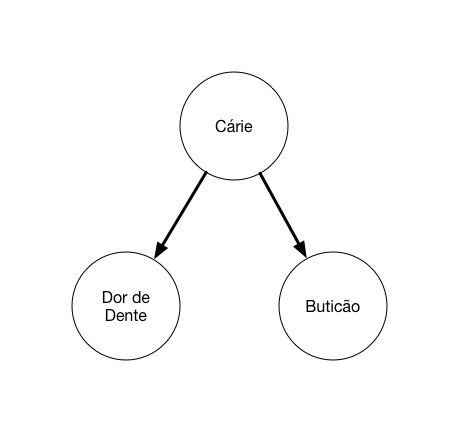
\includegraphics[width=\textwidth]{exemplo_rb}
        \smallcaption{\cite{russell:2002}}
        \label{fig:experimento}
    \end{minipage}
\end{figure}

As setas de conexões entre os nós dão o significado de que os pais influenciam diretamente os filhos. Em termos de causa e efeito, significa que as causas devem ser organizadas como pais dos efeitos~\cite{russell:2002}.

A semântica de uma rede bayesiana pode ser tratada de duas maneiras: (I) a primeira como a representação da distribuição de probabilidade conjunta; (II) a outra, como a codificação de uma coleção de declarações de independência condicional. A primeira é utilizada para compreender a construção da rede, e a segunda em procedimentos de inferência sobre consultas~\cite{russell:2002}.

Quando trata-se da representação da distribuição conjunta total, cada entrada é representada pelo produto dos elementos apropriados das tabelas de probabilidade condicional (TPCs) na rede bayesiana. Dessa forma, a distribuição conjunta total é utilizada para obter respostas sobre qualquer consulta no domínio. Sendo uma rede bayesiana a representação dessa distribuição, ela também obtêm qualquer resposta para consultas sobre o domínio. Para isso, basta efetuar um somatório de todas as entradas conjuntas relevantes~\cite{russell:2002}.

Para que a representação da rede bayesiana sobre um conjunto seja correta, é necessário cada nó ser condicionalmente independente de seus predecessores após a sua ordenação, dados seus pais~\cite{russell:2002}. A seguinte metodologia é aplicada para satisfazer tal condição:

\begin{itemize}
    \item \textbf{Nós}:
    \begin{itemize}
        \item Determinar o conjunto de variáveis que são necessárias para modelar o domínio.
        \item Ordene-as $\{ X_1, \dots, X_n\}$. Não é necessário estabelecer uma ordem específica. Qualquer ordem funciona. Contudo, a rede poderá ser mais compacta, caso a ordem seja feita com as causas sendo os pais dos efeitos.
    \end{itemize}
    \item \textbf{Vínculos}: Para $i = 1$ até $n$ faça:
    \begin{itemize}
        \item Escolha, de $X_1, \dots, X_n$, um conjunto mínimo de pais para $X_i$, tal que a equação~\ref{eq:regra-cadeia} seja satisfeita.
        \item Para cada pai insira um vínculo do pai para $X_i$.
        \item \textbf{TPCs}: escreva a tabela de probabilidade condicional, $P(X_i|Pais(X_i))$
    \end{itemize}
\end{itemize}

\begin{equation}
    \label{eq:regra-cadeia}
    P(X_i|X_{i-1},\dots,X_1) = P(X_i|Pais(X_i)),
\end{equation}

desde que $Pais(X_i) \subseteq \{X_{i-1},\dots,X_1\}$~\cite{russell:2002}.

Após o procedimento, é obtido os pais do nó $X_i$ que contém todos os nós em $X_1, \dots, X_{i-1}$ que possuem influência direta em $X_i$. Esse método de construção da rede garante que ela seja acíclica, uma vez que cada nó é ligado apenas aos seus anteriores~\cite{russell:2002}.

Uma maneira de garantir a consistência da construção da rede bayesiana, é fazer com que ela não possua valores de probabilidade rendundantes ao longo de seus nós. Além disso, a rede bayesiana, em termos computacionais, é mais compacta ao se comparar com a distribuição conjunta total. Assim, o crescimento das variáveis de um domínio, não exercem grandes problemas durante o processo computacional de consultas~\cite{russell:2002, faceli:2011}.

Pode-se dizer também que um nó tem uma independência condicional de todos os outros nós da rede, dados os seus pais, filhos e pais dos filhos, ou seja, dada a cobertura de Markov. Em regras gerais, a relação de pai e filho pode ser descrita como uma distribuição canônica ajustavél a um certo padrão ou forma. Assim, a partir de alguns poucos paramêtros é possível obter a tabela de probabilidade condicional. Essa abordagem facilita, pois diminui a quantidade de números informados à rede~\cite{russell:2002}.

Uma distribuição canônica pode ser exemplificada através de um nó determinístico na rede. Esse tipo de nó tem o valor especificado, exclusivamente, pelos valores dos pais e sem nenhuma incerteza envolvida. Outro exemplo, é um nó numérico como, por exemplo, o nó filho ter atribuido o valor mínimo dentre todos os seus nós pais. Também pode-se aplicar aos nós filhos a soma dos fluxos de entrada subtraídos pelos fluxos de saída~\cite{russell:2002}.

Porém, não é possível atribuir sempre valores certos aos nós da rede bayesiana. Dessa maneira, é necessário trabalhar com relacionamentos de incerteza. Esse tipo de relacionamento é caracterizado por relações de lógica ruidosas. Tais relações são chamadas de ou-ruidoso. O modelo ou-ruidoso permite que a incerteza as condições do pai faça que o filho torne-se verdadeiro. A situação colocada pelo modelo, faz com que o relacionamento causal pai-filho possa ser inibido. Este modelo trabalha com duas suposições~\cite{russell:2002}:

\begin{itemize}
    \item todas as causas possíveis estão pressupostamente listadas. Pode-se considerar nós de vazamento, caso isso não ocorra.
    \item a inibição de cada pai é pressupostamente independente de quaisquer outro pai.
\end{itemize}

A partir das informações acima, é possível construir a tabela de probabilidade condicional inteira. Para isso, utiliza-se a regra geral dada pela equação~\ref{eq:regra-geral}~\cite{russell:2002}.

\begin{equation}
    \label{eq:regra-geral}
    P(x_i|pais(X_i)) = 1 - \prod_{\{j:X_j = verdadeiro\}} ,
\end{equation}

onde o produto é obtido dos pais que são definidos como verdadeiro para cada linha da tabela de probabilidade condicional. Os relacionamentos lógicos ruidosos podem ser descritos com $O(k)$ parâmetros, ao invés de $O(2^k)$ da TPC completa, considerando $k$ pais~\cite{russell:2002}.

% \subsubsection{Métodos de Inferência}
% Quando obtêm-se uma observação de um evento qualquer, dentro de um domínio, espera-se que o sistema de inferência seja capaz de calcular a distribuição de probalidade posterior para o conjunto de variáveis de consulta. Essa é sua tarefa básica. Ele deve atribuir valores ao conjunto de variáveis de evidência~\cite{russell:2002, faceli:2011}.
%
% Um algoritmo utilizado para inferência é o por enumeração. Ele calcula soma-produtos das probabilidades condicionais na rede. Contudo, esse algoritmo pode ser melhorado substancialmente ao eliminar os cálculos repetidos. A ideia de eliminar cálculos funciona da seguinte maneira, após a execução do cálculo pela primeira vez, armazena-se os resultados para futura utilização. É a idéia básica da programação dinâmica. O algoritmo que apresenta a menor complexidade para essa tarela é chamado de algoritmo de eliminação de variáveis (vide algoritmo~\ref{alg:eliminacao-variaveis})~\cite{russell:2002}.
%
% \begin{algorithm}
%     \textbf{função} ASK-ELIMINACAO($X$, \textbf{e}, \emph{rb}) \Retorna uma distribuição sobre $X$
%
%     \Entrada{
%             \begin{tabular}{l}
%                 $X$, a variável de consulta \\
%                 \textbf{e}, variáveis observadas da variável \textbf{$E$} \\
%                 \emph{rb}, uma rede bayesiana especificando a distribuição conjunta $P(X_1, \dots, X_n)$
%             \end{tabular}
%     }
%     \emph{fatores} $\gets$ [ ]
%
%     \ParaCada{var \emph{\textbf{em}} ORDEM(rb.\emph{VARS)}}{
%     \emph{fatores} $\gets$ [CRIAR-FATOR(\emph{var}, \textbf{e})\emph{fatores}]
%
%     \Se{var \emph{é uma variável oculta}}{\emph{fatores} $\gets$ SOMAR(\emph{var}|\emph{fatores})}
%     }
%     \Retorna NORMALIZAR(PRODUTO-PONTUAL(\emph{fatores}))
%     \caption{Algoritmo de eliminação de variáveis para inferência nas redes bayesianas~\cite{russell:2002}}
%     \label{alg:eliminacao-variaveis}
% \end{algorithm}
%
% Esse algoritmo realiza a seguinte verificação: se uma variável não é ancestral de nenhuma variável de consulta ou evidência, essa torna-se irrelevante para o processo. Isso faz com que essa varíavel possa ser eliminada dos cálculos de inferência~\cite{russell:2002}.

Métodos que utilizam a probabilidade de Bayes, são utilizados para diversas tarefas e não apenas tomada de decisão e inferência, mas também classificação, entre outras. Nas seções seguintes são apresentados dois algoritmos para classificação bayesiana.

\subsection{Classificador Naïve Bayes}
\label{sec:naivebayes}

Em um problema onde os valores dos atributos possuem uma independência entre si, a probabilidade $P(x|y_i)$ pode ser decomposta como $P(x_1|y_i) \times \dots \times P(x_d|y_i)$. A equação~\ref{eq:naivebayes} apresenta a probabilidade de um exemplo pertencer à classe $y_i$~\cite{faceli:2011}.

\begin{equation}
    \label{eq:naivebayes}
    P(y_i|x) \propto P(y_i) \prod_{j=i}^{d}P(x_j|y_i)
\end{equation}

Todos os dados para classificar uma classe $y_i$ são obtidos através de um conjunto de treinamento. Os conjuntos que formam as variáveis devem ser discretizados e não continuos. Um classificador naïve bayes é sempre utilizado quando não existe dependência condicional entre as variáveis. Caso exista essa dependência condicional, outras técnicas devem ser utilizadas, como o uso de redes bayesianas. Apesar da recomendação, em alguns casos em particular, o classificador naïve bayes consegue realizar o processo de classificação~\cite{faceli:2011}.

\subsection{Classificação com Redes Bayesianas}
\label{sec:rbclassificador}

A classificação através de uma rede bayesiana é um processo relativamente simples. O primeiro passo para realizar o processo de classificação é determinar uma variável aleatória como alvo, sendo que as demais viram entradas do sistema. Todo o conjunto de variáveis que afetam a variável alvo, pais e filhos da variável alvo, e pais dos filhos da variável alvo é conhecido como \emph{Markov Blanquet}. A partir desse momento a rede bayesiana pode ser utilizada como um classificador, onde dado um exemplo $x$, fornece a probabilidade \emph{a posteriori} $P(y | x)$ do nó classe $y \in Y$. É possível calcular a probabilidade \emph{a posteriori} $P(y|x,S)$ para cada classe $y \in Y$ realizando a marginalização da distribuição de probabilidade conjunta $P(y,x|S)$, onde busca-se o retorno que maxima a classe $\hat{y}$ de acordo com a equação~\ref{eq:crb}~\cite{faceli:2011}.

\begin{equation}
    \label{eq:crb}
    \hat{y} = h_{CRB}(x) = \arg \max_{j=1 \dots k} P(y_j, x | S)
\end{equation}

Na seção a seguir, alguns trabalhos utilizando classificadores bayesianos são apresentados com temas referentes a perfis de usuários e interação humano-robô.

\subsection{Aplicações com Classificadores Bayesianos}
\label{sec:cbrw}
Nessa tese é realizado a proposta de um classificador de perfil do usuário. Esse perfil do usuário é construído no formato de Personas. Sabe-se que determinar um perfil de acordo com o comportamento do usuário é algo que gera uma incerteza. Sendo assim, a técnica mais apropriada para realizar a tarefa é a rede bayesiana, pois é uma técnica probabilística e consegue determinar uma relação condicional entre as características observadas. Nessa seção, classificadores bayesianos são analisados com o intuíto de auxiliar na construção e análise do proposto por essa tese.

Um sistema de visão computacional que realiza a modelagem e análise de interação entre seres humanos, de maneira a entender o que está acontecendo em um cenário de vigilância é apresentado por \citeonline{oliver:2000}. Alguns cenários avaliados são: seguir uma pessoa, alterar o caminho para ir de encontro a outra pessoa, entre outros.

Dois modelos foram utilizados para realizar a classificação do comportamento do usuário nas interações: Hidden Markov Models~(HMM) e o Coupled Hidden Markov Models~(CHMM). O segundo demonstrou-se mais acertivo ao analisar os cenários em videos de auto estradas com agentes sintéticos transitando pelas cenas de um simulador~\cite{oliver:2000}.

O uso de raciocínio baseado em casos para obtenção de características do usuário para formação de um perfil é o trabalho apresentado por \citeonline{schiaffino:2000}. As informações armazenadas são utilizadas para a criação de uma rede bayesiana que analiza os itens de interesse do usuário. Essa técnica é utilizada em um cenário particular de rotina e mudança de comportamento do usuário ao longo do tempo. Assim é possível identificar pontos de mudança na preferência do usuário.

\citeonline{cohen:2003} apresenta a comparação entre três classificadores bayesianos: Naïve Bayes~(NB), Tree Augmented Naïve Bayes~(TAN) e Rede Bayesiana Hierarquica~(RB). O objetivo é identificar expressões faciais a partir da entrada de videos continuos. Os resutaldos demonstram que a RB obteve o melhor resultado com 75\% de acertos, seguido pelo TAN com 73\% e por fim, o NB obteve 72,5\%. Uma extensão do trabalho é apresentado em \citeonline{cohen:2004}, onde é aplicado uma classificação semi-supervisionada para detecção de expressões faciais.

Uma metodologia para estimativa da posição corporal é apresentado por \citeonline{park:2004}. Uma rede bayesiana recebe informações da estimativa do corpo de duas pessoas e a partir dessas informações é feito uma classificação para identificar o que a pessoa está fazendo como, apontando o dedo, brigando, de mãos dadas, chutando, empurrando ou abraçando. A média de acerto na classificação do algoritmo é de 78\% o que foi considerado um sucesso pelos autores.

Redes bayesianas classificando expressões faciais, detecção de faces e peles a partir de um treinamento com informações rotuladas e não rotuladas são criadas por \citeonline{sebe:2005} e \citeonline{sebe:2005b}. Dentre os resultados positivos dos trabalhos, o mais citado foi como as informações não rotuladas auxiliaram na melhora da classificação das RB.

Uma rede bayesiana hierárquica é construída para auxiliar em um sistema de recuperação de arquivos com base no perfil do usuário. O problema encontrado nesse tipo de aplicação é que os usuários novos não possuem uma base para recomendação dos arquivos adequados ao seu perfil. Assim, a rede bayesiana foi construída de maneira a utilizar informações de uso dos antigos usuários para sugerir ao novos usuários arquivos de seu interesse. O sistema conseguiu atingir com sucesso a informações necessárias na recomendação dos arquivos aos novos usuários. Para isso, foi utilizado informações de \emph{feedback} implícito (de acordo com o uso do usuário) e explícito (favoritação dos arquivos)~\cite{zigoris:2006}. O perfil de usuário utilizado neste trabalho é baseado na navegação pelos documentos que o usuário deseja consultar. Nesta tese, o perfil tem como base para sua classificação as informações de interação entre humano e robô.

Uma comparação de quatro algoritmos para a classificação de perfis de usuários é realizada por \citeonline{cufoglu:2008}. Os algoritmos selecionados são: Naïve Bayes~(NB), Rede Bayesiana~(RB), Lazy Learning of Bayesian Rules~(LBR) e Instance-Based Learner~(IB1). Os perfis classificados eram compostos pelas seguintes informações: idade, classe de trabalho, educação, estado civil, ocupação, relacionamento, etnia, gênero, país nativo.

Os algoritmos que demonstraram os melhores resultados foram NB e IB1 que obteveram a mesma precisão na classificação, 95\% de acurácia. O LBR apresentou uma acurácia de 94,7\%, seguido pela RB com 94,4\%. A continuação do trabalho é a comparação com classificadores mais clássicos como \emph{Support Vector Machines}~(SVM) e árvores de decisão~\cite{cufoglu:2008}.

Outra comparação é proposta no trabalho de \citeonline{iglesias:2008}. A comparação entre três métodos para classificar o perfil de comportamento do usuário no uso do sistema operacional UNIX. Os métodos utilizados são: RB, HMM e \emph{Term Frequency Inverse Document Frequency}~(TFIDF). Como entrada da classificação do comportamento é utilizado a sequência de comandos inseridas no terminal pelo usuário. TFIDF apresentou uma média de 57,1\% de acerto na classificação, a RB apresentou 44,2\% e o HMM com o melhor índice conseguiu uma taxa de acerto de 76,4\% snedo o mais indicado para o cenário de aplicação testado.

É proposto por \citeonline{prado:2012} um método para analizar e sintetizar faces e voz com o objetivo de reconhecer emoções do usuário. Posteriormente essas informações são inseridas em um estrutura de rede bayesiana onde é feito o trabalho para classificar essas emoções. A partir da classificação o robô pode tomar a decisão de reação adequada a interação.

\citeonline{escalante:2016} apresentam um classificador naïve bayes para identificar gestos e ações do usuário através de entradas de frames de videos. Outra maneira de utilizar o classificador naïve bayes é apresentada por \citeonline{liu:2016}. Um método de aprendizado por observação de gestos e fala em interações humano-robô. Esse método é aplicado em um cenário de interação de compra em loja de produtos simuladas. Para realizar o aprendizado, \citeonline{liu:2016} realizaram o agrupamento das informações sobre a interação e alimentaram o classificador naïve bayes, resultando no aprendizado do robô. Conceitos de \emph{Proxemics} também foram utilizados para auxiliar a determinar o espaço das interações face a face. O comportamento do robô teve uma acurácia de 84,8\% enquanto a parte de voz obteve apenas 76,8\% de aproveitamento.

Técnicas de classificação probabilísticas tem demonstrado grande aplicabilidade dentro de trabalhos com perfis de usuário e interação humano-robô e humano-computador. Porém é importante mencionar que, nenhum trabalho aplicou na classificação bayesiana alguma técnica no contexto de experiência de usuário. A classificação bayesiana pode auxiliar no projeto de interação humano-robô, pois pode apoiar o processo autonômo de adaptação do comportamento do robô no cenário de robótica social.
